\section{Resonators}
\label{sec:theory.resonator}

\subsection{A generic model for a shunt-coupled resonator}
\label{sec:theory.resonator.generic}

To understand KID response we need to understand how the behavior of a superconducting resonator will change when the surface impedance shifts in some region of the resonator.
A specific resonator geometry can be analyzed using circuit concepts such as capacitance and inductance.
However, since many different resonator geometries can be used for KIDs, I begin by introducing a generic resonator model.

The two relevant frequencies are the fixed readout tone frequency $\freadout_\readout$ and the variable resonance frequency $\freadout_\resonator$.
There are advantages to using lower readout frequencies, so KIDs are typically read out at their fundamental resonance.
Decreasing this frequency generally requires more area, which is a precious quantity at the focal plane of a telescope.

In order to compare resonators with very different resonance frequencies, it is more convenient to use dimensionless variables.
The fractional frequency shift is
$\shift = 1 - \freadout_\resonator / \freadout_\resonator^\zerotemp$,
where $\freadout_\resonator^\zerotemp$ is the resonance frequency in some fiducial state, such as temperature approaching zero.
One could measure this shift directly by tracking the resonance frequency in real time.
However, our readout system can measure this shift directly only by sweeping the readout tone across a resonance, as shown in Figures~\ref{fig:introduction_resonator_amplitude_phase}~and~\ref{fig:example_resonator_fit_amplitude_phase_and_normalized}.
This method is slow, and we thus measure $\shift$ only in steady-state.
A simple readout technique is to sweep a tone across a resonance,  use a resonator model to determine the resonance frequency, then  set a single tone at this frequency and sample rapidly.
With this technique, the dimensionless quantity measured when obtaining time-ordered data is the fractional frequency detuning
$\detuning = \freadout_\readout / \freadout_\resonator - 1$ of the resonance frequency from the readout frequency.
We set $\freadout_\readout$ as close to $\freadout_\resonator$ as the readout electronics allow, and typically $\detuning < \num{e-5}$.
The fractional frequency shift and the detuning are clearly closely related: to a very good approximation, a shift $\delta\shift$ corresponds to an equal shift $\delta\detuning$.
Generally, I will use $\shift$ when describing steady-state measurements and will use $\detuning$ when describing time-ordered data.
The signs of these parameters are chosen so that when the resonance frequency $\freadout_\resonator$ decreases, as it does under increasing illumination, the dimensionless parameter increases.

Additional parameters characterize the flow of energy in the resonator.
The quality factor of a resonator is defined to be the ratio of energy stored to the energy lost per radian of oscillation.
The latter equals the power lost divided by the angular oscillation frequency, which is typically very close to the resonance frequency, so the resonator quality factor is
\begin{equation}
\qf_\resonator
  =
  \frac{2 \pi \freadout_\resonator \energy_\mathrm{stored}}{\power_\mathrm{out}}.
\end{equation}
We distinguish between two mechanisms for energy loss: $\power_\mathrm{out}$ includes both dissipation internal to the resonator and loss due to radiation back onto the feedline:
\begin{equation}
\qf_\resonator^{-1}
  \equiv
  \loss_\resonator
  =
  \loss_\coupling + \loss_\internal
  \equiv
  \qf_\coupling^{-1} + \qf_\internal^{-1},
\end{equation}
where $\loss = \qf^{-1}$ is a notational convenience I will use repeatedly.
The inverse quality factor, which I refer to as a ``loss,'' is easier to work with, but quality factors are conventional.

Thus, the internal loss $\loss_\internal = \qf_\internal^{-1}$ characterizes dissipation in the resonator, and an increase in the quasiparticle number causes the internal loss to increase.
As discussed further in Chapter~\ref{chp:loss}, the internal loss also includes various non-ideal sources of loss, such as dissipation in dielectrics, radiation into free space, and dissipation caused by vortices in the superconducting film.
The coupling loss $\loss_\coupling = \qf_\coupling^{-1}$ characterizes the coupling strength between the resonator and the feedline.

An additional nuisance parameter, the asymmetry parameter $\asymmetry$, is necessary to characterize a commonly-occurring resonance asymmetry that can be caused either by parasitic coupling between the resonator and the feedline or by an impedance mismatch between the feedline and the transmission lines to which it connects~\autocite{Khalil2012JAP}.
For a symmetric resonance, $\asymmetry = 0$.

\todo[inline]{Understand coupling quality factor and radiation}
%This radiated power is assumed to propagate equally in both directions along the feedline until it is absorbed by matched resistive loads.
%Radiation propagating toward the low-noise amplifier is absorbed and amplified, while radiation propagating in the other direction is presumably absorbed by some matched load in the input chain.

KIDs are read out in the in the shunt-coupled configuration shown in Figure~\ref{fig:multiplexed_mkids_v1}.
It is convenient to express the measured transmission past the resonators in terms of the forward scattering parameter
$\forwardscattering = \voltage_2 / \voltage_1$,
where $\voltage_1$ and $\voltage_2$ are the complex voltages on the feedline of, respectively, the wave propagating toward the resonators and the wave arriving at the low-noise amplifier.
(The readout system actually records this quantity multiplied by the complex gain $G$ of the system:
$R_{21} = G \forwardscattering$.)
In terms of the parameters defined above, the forward scattering response due to one resonator is
\begin{equation}
\forwardscattering(\freadout_\readout, \freadout_\resonator, \loss_\internal, \loss_\coupling, \asymmetry)
  =
  1 - \frac{1 + \I \asymmetry}{1 + (\loss_\internal + 2 \I \detuning) / \loss_\coupling},
\label{eqn:forwardscattering}
\end{equation}
which is equivalent to the more familiar form~\autocite{Zmuidzinas2012ARCMP}
\begin{equation}
\forwardscattering(\freadout_\readout, \freadout_\resonator, \qf_\resonator, \qf_\coupling, \asymmetry)
  =
  1 - \frac{\qf_\resonator (1 + \I \asymmetry) / \qf_\coupling}{1 + 2 \I \qf_\resonator \detuning}.
\end{equation}
Figure~\ref{fig:example_resonator_fit_amplitude_phase_and_normalized} shows forward scattering data with the readout tone swept across the resonance frequency and a fit to Equation~\ref{eqn:forwardscattering}.
In time-ordered data collected at a fixed readout frequency the quantities that vary in time are $\loss_\internal$ and $\freadout_\resonator$ (and thus $\detuning$), while  
$\loss_\coupling$ and $\asymmetry$ do not vary.

\begin{figure}[tb]
\centering
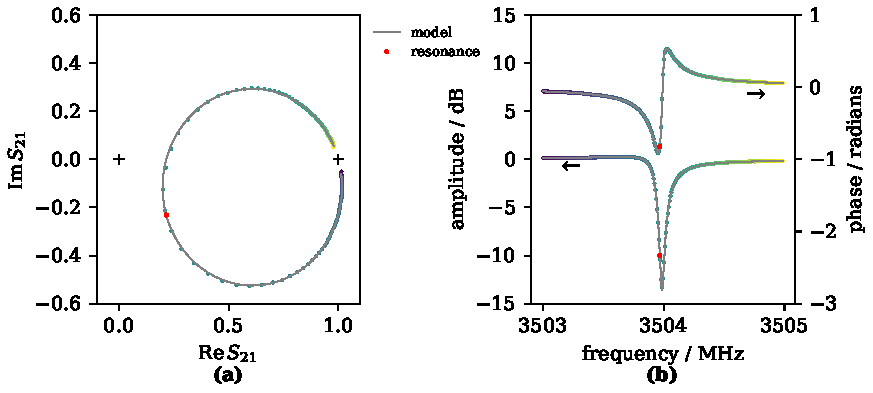
\includegraphics[width=\textwidth]{theory/example_resonator_fit_amplitude_phase_and_normalized.pdf}
\caption
[Complex transmission data from a frequency sweep across a resonator, normalized and fit to a resonator model.]
{
Complex transmission data from a frequency sweep across a resonance.
The resonator model given in Equation~\ref{eqn:forwardscattering} was fit to the data, and the points were normalized by dividing out the system gain.
The device is an aluminum CPW resonator with a resonance frequency near \SI{3.5}{GHz}.
In both panels, the purple (yellow) points correspond to the low (high) end of the frequency sweep, which spans \SI{2.0}{MHz}.
\textbf{(a)} 
The frequency sweep data and model in the complex $\forwardscattering$ plane.
The + symbols mark (0, 0) and (0, 1), which the model constrains the data to approach far from the resonance.
The internal loss is
$\loss_\internal = \num{8.9e-6} = 1 / \num{1.1e5}$,
and the coupling loss is
$\loss_\coupling = \num{3.2e-5} = 1 / \num{3.1e4}$.
This resonance has a relatively large value of the asymmetry parameter
$\asymmetry = 0.3$, which causes the resonance circle to be rotated and expanded.
\textbf{(b)} 
The same data and model plotted versus frequency, with amplitude on the left axis and phase on the right axis.
Because of the large asymmetry, the resonance frequency does not appear to be at the center of the amplitude or phase curves.
}
\label{fig:example_resonator_fit_amplitude_phase_and_normalized}
\end{figure}


\subsection{The effective kinetic inductance fraction}
\label{sec:theory.resonator.kifraction}

To model KID response, we must relate changes in the resonator parameters introduced above to changes in the film surface impedance in the region where quasiparticles are generated.
The two resonator geometries used in this thesis are lumped-element resonators and quarter-wave transmission-line resonators.

We begin with the simpler case of a lumped-element resonator. 
Figures~\ref{fig:loss.experiment}~and~\ref{fig:measuring.experiment} show drawings of aluminum lumped-element resonators, which consist of a meandered inductive trace and an interdigital capacitor that are both electrically short at the resonance frequency.
For these devices, the resonance frequency is
$\freadout_\resonator
  =
  (2 \pi)^{-1} (\inductance \capacitance)^{-1/2}$
where $\inductance$ is the total inductance of the resonator and $\capacitance$ is its total capacitance.
The total inductance
$\inductance = \inductance_\geometric + \inductance_\kinetic$
is the sum of the geometric inductance $\inductance_\geometric$ and the kinetic inductance $\inductance_\kinetic$, where $\reactance_\surface = 2 \pi \freadout \inductance_\kinetic$.
The response to an inductance shift in some region is weighted by the square of the current in that region~\autocite{Mazin2005,Gao2008}.
For these resonators, the current is approximately constant along the inductive meander and is very small in the capacitor.
Assume that quasiparticles cause a homogeneous shift in the surface impedance of the inductor.
Then, a small shift in the kinetic inductance
$\inductance_\kinetic - \inductance_\kinetic(0)$ from the zero-temperature value $\inductance_\kinetic(0)$ produces a new resonance frequency
\begin{equation}
\freadout_\resonator
  \approx
  \freadout_\resonator(0)
  \left( 1 - \frac{\inductance_\kinetic - \inductance_\kinetic(0)}{2 [\inductance_\geometric + \inductance_\kinetic(0)]} \right)
  \equiv
  \freadout_\resonator(0)
  \left( 1 - \frac{\kifraction}{2} \frac{\inductance_\kinetic - \inductance_\kinetic(0)}{\inductance_\kinetic(0)} \right).
\end{equation}
Here, the effective kinetic inductance fraction is
\begin{equation}
\kifraction
  =
  \frac{\inductance_\kinetic(0)}{\inductance_\geometric + \inductance_\kinetic(0)}
  =
  \frac{\reactance_\surface(0)}{\reactance_\geometric + \reactance_\surface(0)},
\end{equation}
where $\reactance_\geometric = 2 \pi \freadout \inductance_\geometric$.
In this simple case, the effective kinetic inductance fraction actually equals the ratio of the kinetic inductance to the total inductance, but this is not true when the surface impedance does not shift homogeneously.

The corresponding fractional frequency shift is
\begin{equation}
\shift
  =
  \frac{\kifraction}{2} \frac{\reactance_\surface - \reactance_\surface(0)}{\reactance_\surface(0)}.
\end{equation}
The approximations used here should be quite good in practice: for the lumped-element detectors discussed
in Chapter~\ref{chp:sensitivity}, the total fractional frequency shift between no illumination and very high illumination is $\shift < \num{e-3}$.
Thus, all three of the frequencies $\freadout_\readout$, $\freadout_\resonator$, and $\freadout_\resonator(0)$ are very close to each other so $\kifraction$ can be treated as a constant.

Attributing all dissipation that occurs within the film to quasiparticles, the quasiparticle loss is~\autocite{Zmuidzinas2012ARCMP}
\begin{equation}
\loss_\quasiparticle
  =
  \qf_\quasiparticle^{-1}
  =
  \kifraction \frac{\resistance_\surface}{\reactance_\surface(0)}.
\label{eqn:resonator.loss_quasiparticle}
\end{equation}

The hybrid co-planar waveguide (CPW) KIDs discussed in Chapter~\ref{chp:multichroic} consist of two different sections of CPW in series.
The section closest to the transmission line is made from a high-gap superconductor in which no quasiparticles are excited.
The other section consists of an aluminum center strip that is electrically connected to the high-gap superconductor center strip at one end and to the ground plane at the other end.
The total length is a quarter wavelength at the fundamental resonance frequency.
The quasiparticles are confined to the aluminum region of the center strip, called the active region, where the current is highest.
Thus, only the surface impedance in the active region is altered.
For these resonators we can use the same equations as above with the geometric complications folded into the effective kinetic inductance fraction~\autocite{Gao2008}.
\todo[inline]{Incorporate Jiansong's work on hybrid resonators and on transmission-line resonators with an arbitrary terminating impedance.}
